% Options for packages loaded elsewhere
\PassOptionsToPackage{unicode}{hyperref}
\PassOptionsToPackage{hyphens}{url}
%
\documentclass[
]{book}
\usepackage{amsmath,amssymb}
\usepackage{lmodern}
\usepackage{iftex}
\ifPDFTeX
  \usepackage[T1]{fontenc}
  \usepackage[utf8]{inputenc}
  \usepackage{textcomp} % provide euro and other symbols
\else % if luatex or xetex
  \usepackage{unicode-math}
  \defaultfontfeatures{Scale=MatchLowercase}
  \defaultfontfeatures[\rmfamily]{Ligatures=TeX,Scale=1}
\fi
% Use upquote if available, for straight quotes in verbatim environments
\IfFileExists{upquote.sty}{\usepackage{upquote}}{}
\IfFileExists{microtype.sty}{% use microtype if available
  \usepackage[]{microtype}
  \UseMicrotypeSet[protrusion]{basicmath} % disable protrusion for tt fonts
}{}
\makeatletter
\@ifundefined{KOMAClassName}{% if non-KOMA class
  \IfFileExists{parskip.sty}{%
    \usepackage{parskip}
  }{% else
    \setlength{\parindent}{0pt}
    \setlength{\parskip}{6pt plus 2pt minus 1pt}}
}{% if KOMA class
  \KOMAoptions{parskip=half}}
\makeatother
\usepackage{xcolor}
\usepackage{longtable,booktabs,array}
\usepackage{calc} % for calculating minipage widths
% Correct order of tables after \paragraph or \subparagraph
\usepackage{etoolbox}
\makeatletter
\patchcmd\longtable{\par}{\if@noskipsec\mbox{}\fi\par}{}{}
\makeatother
% Allow footnotes in longtable head/foot
\IfFileExists{footnotehyper.sty}{\usepackage{footnotehyper}}{\usepackage{footnote}}
\makesavenoteenv{longtable}
\usepackage{graphicx}
\makeatletter
\def\maxwidth{\ifdim\Gin@nat@width>\linewidth\linewidth\else\Gin@nat@width\fi}
\def\maxheight{\ifdim\Gin@nat@height>\textheight\textheight\else\Gin@nat@height\fi}
\makeatother
% Scale images if necessary, so that they will not overflow the page
% margins by default, and it is still possible to overwrite the defaults
% using explicit options in \includegraphics[width, height, ...]{}
\setkeys{Gin}{width=\maxwidth,height=\maxheight,keepaspectratio}
% Set default figure placement to htbp
\makeatletter
\def\fps@figure{htbp}
\makeatother
\setlength{\emergencystretch}{3em} % prevent overfull lines
\providecommand{\tightlist}{%
  \setlength{\itemsep}{0pt}\setlength{\parskip}{0pt}}
\setcounter{secnumdepth}{5}
\usepackage{booktabs}
\ifLuaTeX
  \usepackage{selnolig}  % disable illegal ligatures
\fi
\usepackage[]{natbib}
\bibliographystyle{plainnat}
\IfFileExists{bookmark.sty}{\usepackage{bookmark}}{\usepackage{hyperref}}
\IfFileExists{xurl.sty}{\usepackage{xurl}}{} % add URL line breaks if available
\urlstyle{same} % disable monospaced font for URLs
\hypersetup{
  pdftitle={Investigating the effect of different experimental diets and salinities on the growth of Penaeus monodon},
  pdfauthor={Md Rony Golder},
  hidelinks,
  pdfcreator={LaTeX via pandoc}}

\title{Investigating the effect of different experimental diets and salinities on the growth of \emph{Penaeus monodon}}
\author{Md Rony Golder}
\date{2023-06-18}

\begin{document}
\maketitle

{
\setcounter{tocdepth}{1}
\tableofcontents
}
\hypertarget{prerequisites}{%
\chapter*{Prerequisites}\label{prerequisites}}
\addcontentsline{toc}{chapter}{Prerequisites}

This thesis is copyright material protected under the Berne Convention, the Copyright Act 1999 and other international and national enactments, in that behalf, on intellectual property. It may not be reproduced by any means, in full or in part, except for short extracts in fair dealings, for research or private study, critical scholarly review or discourse with an acknowledgement, without the written permission of the Directorate of Postgraduate Studies, on behalf of both the author and the Khulna University

\hypertarget{aknowledgment}{%
\chapter*{Aknowledgment}\label{aknowledgment}}
\addcontentsline{toc}{chapter}{Aknowledgment}

At first, all my admiration goes to the supreme creator and Ruler of the universe, the Almighty
Allah for His great mercy to keep me alive and enables me to pursue my education in Fisheries
and Marine Resource Technology Discipline as well as to complete my work for the degree of
Bachelor of Science in Fisheries.
I would like to express my sincere gratitude and profound appreciation to my honourable
supervisor, Shikder Saiful Islam, Assistant Professor, Fisheries and Marine Resource Technology
Discipline, for his continuous guidance, valuable suggestions, critical observations and sustained
support in writing this thesis.
I would like to express my profound gratitude to Professor Dr.~Ghausiatur Reza Banu, Head,
Fisheries and Marine Resource Technology Discipline, Khulna University for her valuable
suggestions and providence of all necessary facilities.
I recall with warm appreciation and great indebtedness or the support, guidance and suggestions
extended to me by all of my respected teachers in Fisheries and Marine Resource Technology
Discipline, Khulna University.
I would also like to give special thanks to WorldFish, a non-profit research organization for
financial support through Blue Economy Challenge Project to conduct this research for harnessing
the potential of fisheries and aquaculture to strengthen livelihoods and improve food and nutrition
security.
Special thanks goes friends Md. Abdul Kadir Zilany for his support for completing my thesis work
in laboratory.
Finally, I would like to express my very profound gratitude to my parents for all care, unfailing
support and continuous encouragement throughout my study. This accomplishment would not
have been possible without them.

\hypertarget{dedication}{%
\chapter*{Dedication}\label{dedication}}
\addcontentsline{toc}{chapter}{Dedication}

This thesis is dedicated to my beloved parents for their love patience and understanding, who played an important role along this journey, providing encouragement and moral support when it seemed impossible. May Almighty God bless you!

\hypertarget{abstract}{%
\chapter*{Abstract}\label{abstract}}
\addcontentsline{toc}{chapter}{Abstract}

This study evaluates the effect of different salinities and four experimental diets on percent
specific growth rates (\%SGR), weight gain (WG), daily weight gain (DWG), daily growth rate
(DGR), relative growth rate( RGR) and survival of Penaeus monodon. Juveniles of P. monodon
were cultured at salinities of 5, 10, 15, 20, ppt by feeding with four experimental diets (F1, F2, F3
and F4) for 45 days. In this study, the feed's fishmeal protein was replaced with concentrated
microbial protein as an approach to blue economy challenge and aquaculture sustainability. Results
of this study showed that different growth rates of P. monodon were not significantly affected by
four different diets. However, significantly lower \%SGR was observed at 10 ppt, which ranged
from 1.144±1.19 to -0.364±0.53 (P\textless0.05). No significant differences was observed in DGR
(ranged from 10.760±0.08 to -0.253±0.53) as well as in \%RGR (ranged from 378.143±26.03 to -
4.553±20.68) values. In contrast, salinities were found to have a significant effect on the combined
dependent variable (P\textless{} 0.05). However, different feeds, and feed-salinity interaction did not show
any significant effect on the variation of combined dependent variables (P\textgreater0.05). Finally, test of
between subject effects demonstrated that different feeds, salinities, and interaction of feeds and
salinities had no significant effect on the individual dependent variable in different tanks (P\textgreater0.05).
In conclusion, different salinity might affect the culture and production of tiger shrimp in
Bangladesh. Although we did not get any effect but further studies with close observation and with
proper culture facilities different diets might also impact tiger shrimp production.

\hypertarget{introduction}{%
\chapter{Introduction}\label{introduction}}

Bangladesh is blessed with vast and well diversified inland open waters, estuaries, brackish and
marine waters with the potential fisheries resources. Fisheries sector has been playing increasingly
an important role in our economy for few decades (DoF, 2018). Fish is the second most valuable
agricultural crop in Bangladesh and its production contributes to the livelihoods and employment
of millions of people (Ghose, 2014). As an agro-based country, the contribution of fisheries sector
to national economy has always been important and main source of animal protein, employment
opportunities, food and nutritional security, foreign earnings, aquatic biodiversity conservation
and socio-economic development. Fisheries sector contributes 3.61\% to GDP and 24.41\% to
agricultural GDP. Fish supplements to about 60\% of our daily animal protein intake. About 11\%
of the population dependents directly and indirectly on the fisheries sector for their livelihood
(DoF, 2018).

Production of commercial feeds has increased at an average rate of 32\% per year over the period
2008--2012, and has reached an estimated total of almost 1.07 million tons in 2012. Sinking feeds,
which accounted for 81\% of total manufactured output, still dominate over extruded floating feed
(19\%), but growth in the production of floating fish feed has been fastest, averaging 89\% over the
last four years. Around 100 commercial mills produce aquaculture feeds in Bangladesh (Rashid et
al., 2013).

The costs of formulated feed and labor associated with feeding are a major component of the cost
of cultured shrimp production (Lawrence and Lee, 1997). It is well established that the nutrient
contents of the feed influence growth, survival and the amount of metabolic and excreted waste
products entering the system. However, processing also plays a critical role as it influences
stability of the feed and hence availability of the feed over time (Smith, Burford, \& Tabrett, 2002).

Although filter feeding animals like mollusks or herbivorous silver carp and bighead carp do not
require feeding (FAO, 2012b); however, fed aquaculture represents 81 percent of global fish and
crustacean aquaculture production. Fed aquaculture contributes about 60 percent of global aquatic
animal production of aquaculture (Tacon et al., 2013). Although, in developing countries fewer
supplementary feeds and fishmeal are used due to lower trophic level species culture, but for the
higher trophic level species, like shrimp, salmon, trout are still dependent on fish from the wild for fishmeal and oil in formulated feeds (HLPE, 2014). The use of fish from the wild in fishmeal and
fish oil to produce fish has been the cause of major public controversy. In 2012, about 10 percent
of total catch fish (16 million tons) was reduced to fishmeal and fish oil (Tacon et al., 2011; FAO,
2014a). In addition to fishmeal and fish oil, trash fishes are also used directly.

The aquaculture research community and the aquafeeds industry have long recognized and
anticipated issues impacting the sustainability of fish meal in aquafeeds (Barrows and Hardy,
2001) and have been researching and developing aquafeeds that use alternative protein ingredients,
particularly plant-derived proteins (Gatlin et al., 2007). Blue economy challenge project tried to
find an alternative approach of protein source in collaboration with Waginengen University and
Research, WorldFish Bangladesh, Vietnam and Khulna University developed different types of
feeds supplemented with concentrated microbial proteins into shrimp feed. Moreover, most of the
shrimp culture farms at different coastal districts in Bangladesh have been developed at different
salinities. There is a little literature has been found who worked on protein supplementation in
shrimp feed with microbial proteins and its suitability in application at different salinities, and its
performance in growth of \emph{P. monodon}.

\hypertarget{objectives-of-the-study}{%
\section{Objectives of the study}\label{objectives-of-the-study}}

In this BSc thesis attempt was taken to investigate effect of different experimental diets enriched
with concentrated microbial protein and salinities on the growth of P. monodon. The idea was to
understand the compatibility of these experimental diets in the shrimp farms of different coastal
districts of Bangladesh.
The objectives of this study were to:

\begin{itemize}
\tightlist
\item
  Investigate the effect of different experimental diets and salinities on the growth of \emph{P.monodon}.
\end{itemize}

\hypertarget{review-of-literature}{%
\chapter{Review of literature}\label{review-of-literature}}

\hypertarget{overview-of-aquaculture}{%
\section{Overview of aquaculture}\label{overview-of-aquaculture}}

\hypertarget{present-status-of-aquaculture}{%
\subsection{Present status of aquaculture}\label{present-status-of-aquaculture}}

Aquaculture production has grown rapidly over the past four decades,
contributing significant quantities to the world's supply of fish for
human consumption. Aquaculture now accounts for almost 53\% of the
world's food fish. (FAO, 2018). With its continued growth, it is
expected that aquaculture will, in the near future, produce more fish
for direct human consumption than capture fisheries (Subasinghe et al.,
2009). Bangladesh is considered one of the most suitable regions for
fisheries in the world, with the world's largest flooded wetland and the
third largest aquatic biodiversity in Asia after China and India
(Shamsuzzaman et al., 2017) Fish is the second most valuable
agricultural crop in Bangladesh and its production contributes to the
livelihoods and employment of millions of people. The culture and
consumption of fish therefore has important implications for national
income and food security. Bangladeshi people are popularly referred to
as ``Mache Bhate Bangali'' or ``fish and rice makes a Bengali'' (Ghose,
2014).Global production of fish, crustaceans, molluscs and other aquatic
animals continued to grow and reached 169.2 million tonnes in 2015. Of
this total, aquaculture production was 76.6 million tonnes in 2015, up
by 4 percent from previous year. (FAO, 2018).

Bangladesh is one of the world's leading fish producing countries with a
total production of 4.134 million MT in 2016-17, of which inland open
water (capture) contributes 28.14\% and inland closed water (culture)
contributes 56.44\% of total production. Several statistics represented
that the annual growth rate of total fish production in 2016-2017 was
6.60\%. This increasing aquaculture growth rate revealed more than five
times country's aquaculture production (7.54 MT in 1983-84 to 41.34 lakh
MT in 2016-17) over the last three decades Government is trying to
sustain this growth performance, which eventually ensures to achieve the
projected production target of 4.55 million MT by 2020-21. Recently,
Bangladesh has been ranked as the fifth position in world aquaculture
production (DoF, 2017).

The total first sale value of fisheries and aquaculture production in
2016 was estimated at USD 362 billion, of which USD 232 billion was from
aquaculture production.(FAO, 2018). The total production included 80.0
million tonnes of food fish (USD 231.6 billion) and 30.1 million tonnes
of aquatic plants (USD 11.7 billion) as well as 37 900 tonnes of
non-food products (USD 214.6 million). Farmed food fish production
included 54.1 million tonnes of finfish (USD 138.5 billion), 17.1
million tonnes of molluscs (USD 29.2 billion), 7.9 million tonnes of
crustaceans (USD 57.1 billion) and 938 500 tonnes of other aquatic
animals (USD 6.8 billion) such as turtles, sea cucumbers, sea urchins,
frogs and edible jellyfish.

Shrimp is one of the major export items in Bangladesh. This sector is
contributing significantly in food security through proving safe and
quality animal protein; almost 60 percent animal protein comes from
fish. It contributes 3.61 percent to our national GDP and around
one-fourth (24.41 percent) to the agricultural GDP. This sector also has
high potential for the perspective of economic development of the
country. Bangladesh earns a considerable amount of foreign currencies by
exporting fish, shrimps and other fisheries products. Bangladesh exports
frozen shrimp and other fish and fisheries products to more than 50
countries, including Belgium UK, Netherlands, Germany, USA, China,
France, Russian Federation, Japan and Saudi Arabia. In 2016-17, the
country earns BDT 42876.40 million by exporting almost 68.31 thousand MT
of fish and fisheries products. This success is due to export of quality
shrimp introducing HACCP procedure and traceability regulation according
to the requirement of European Union (EU) and USA (DoF, 2017).

\begin{figure}
\centering
\includegraphics{https://www.fao.org/3/cc0461en/online/sofia/img/CC0461EN_SOFIA_fig13.jpg}
\caption{Figure 1 World Aquaculture production (FAO,
2018)}
\end{figure}

Aquaculture contribute significantly for the livelihood of a huge number
of people, for instance about 56.5 million people were engaged in the
primary sector of capture fisheries (67) and aquaculture (33\%). In
addition, this sector brought women at nearly 19\% of the primary
workforce (FAO, 2017). More than 11 percent of total population of
Bangladesh are engaged with this sector either on full time or part time
basis for their livelihoods (DoF, 2017).

Commercial shrimp feed constitutes 50--60\% operational cost of intensive
shrimp farming (Wasielesky et al., 2006). So, formulation of
nutritionally balanced feed with quality dietary supplement is an
imperative area of research to meet the nutritional demand and maximize
the growth of shrimp. Most commonly used dietary supplements in penaeid
shrimp diets are microalgae (Ju et al., 2009; Supamattaya et al., 2005),
seaweed (Yeh et al., 2006), herbal extract (Sankar et al., 2011), yeast
(Yang et al., 2010), probiotics (Wang, 2007; Ziaei-Nejad et al., 2006),
carotenoids (Boonyaratpalin et al., 2001) and prebiotics (Zhang et al.,
2012). (Anand et al., 2013). The domestic source of better quality fish
meal (44--52\% crude protein content) is the chewa (Pseudapocryptes
elongates), supplied in southern Bangladesh in Kuakata and the islands
of Hatia and Bohala, but amounts available are insufficient to meet the
demand of the feed sector. An approximate calculation indicates that the
annual catch of fresh trash fish is close to 0.15 million tonnes; equal
to approximately 0.0375 million tonnes of fish meal. Considering that
most feed producers aim for at least 5\% inclusion of fish meal, this
quantity of supply is insufficient to meet demand. (Rashid et al.,
2013).

\hypertarget{problems-in-aquaculture}{%
\section{Problems in Aquaculture}\label{problems-in-aquaculture}}

\hypertarget{general-problems}{%
\subsection{General Problems}\label{general-problems}}

Under good management, several technical difficulties may arise during
fish culture with a possibility of large scale loss of production. Some
of such common difficulties in fish ponds/ fish culture are- Deep green
water color, muddy pond water, red layer on pond water, oxygen depletion
in pond water and fish grasping for air, excess ammonia, hydrogen
sulphide, dark mud at bottom, larger aquatic plants in pond and so on
(Hussain et al., 2016)

\hypertarget{diseases}{%
\subsection{Diseases}\label{diseases}}

The diseases of cultured penaeid shrimp include syndromes with
infectious and non-infectious etiologies. The common infectious diseases
which cause significant economic loses in shrimp culture are with viral,
rickettsial, bacterial, fungal, protistan and metazoan etiologies
(Lightner, 1988, 1993a, 1996; Brock and Lightner, 1990; Fulks and Main,
1992; Johnson, 1995). A number of noninfectious diseases are also of
importance to the industry, and included among these are diseases due to
environmental extremities, nutritional imbalances, toxicants, and
genetic factors (Lightner, 1988; Brock and Lightner, 1990b; Brock, 1992;
Johnson, 1995; Lightner, 1996).

Table 1.1 Major diseases of IndoPacific and east Asian penaeid shrimp
(Lightner \& redman, 1998).

\begin{longtable}[]{@{}lll@{}}
\toprule()
Viral diseases & Bacterial and fungal & Other diseases \\
\midrule()
\endhead
White spot group & Vibriosis: & Epicommensals \\
Yellow head virus & -Septic HP necrosis & - Leucothrix mucor \\
BMN group & -Hatchery vibriosis & - Peritrich protozoans \\
MBV group & -Luminescent Vibrio & Gregarines \\
IHHNV & Rickettsia & Microsporidians \\
HPV & Larval mycosis & Nutritional imbalances \\
REO group & Fusariosis & Toxic syndromes \\
& & Environmental syndromes \\
& & One month death syndrome \\
\bottomrule()
\end{longtable}

\hypertarget{environmental-problem}{%
\subsection{Environmental problem}\label{environmental-problem}}

Land-based fish farms live in tanks containing dirty water that must be
changed. Depending on the system's set-up, this can result in the
discharge of significant amounts of wastewater containing feces,
nutrients and chemicals released into the environment. The release of
this matter can result in algae blooms which eventually remove dissolved
oxygen in the receiving waterway (Michael, 2018).

\hypertarget{development-of-shrimp-feed}{%
\section{Development of Shrimp feed}\label{development-of-shrimp-feed}}

\hypertarget{overview-of-feed-production}{%
\subsection{Overview of feed production}\label{overview-of-feed-production}}

Production of commercial feeds has increased at an average rate of 32\%
per year over the period 2008--2012, and has reached an estimated total
of almost 1.07 million tonnes in 2012. Sinking feeds, which accounted
for 81\% of total manufactured output, still dominate over extruded
floating feed (19\%), but growth in the production of floating fish feed
has been fastest, averaging 89\% over the last four years. Around 100
commercial mills produce aquaculture feeds in Bangladesh. (Rashed et
al., 2013).

\hypertarget{alternative-protein-sources}{%
\subsection{Alternative protein sources}\label{alternative-protein-sources}}

\hypertarget{replacement-with-plant-protein}{%
\subsection*{Replacement with plant protein}\label{replacement-with-plant-protein}}
\addcontentsline{toc}{subsection}{Replacement with plant protein}

Fish meal is currently one of the major sources of animal protein used
in diets for marine shrimp (Sá et al., 2013). Protein is the most
expensive ingredient in the diet, and its quality is a very important
nutritional aspect in aquaculture (Gomez et al., 2008). Fish meal
production has declined by an average of 1.7\% per year over the past 15
years (1994-2009), limiting the supply of this input and thus increasing
its cost (FAO, 2012). This reality can make the production of many
aquatic species economically unfeasible. Among the plant protein
sources, soybean protein concentrate and soybean meal are noteworthy
because of the wide availability of soybeans in the market. However,
soybean protein concentrate is a more refined protein source, with up to
65\% protein content and a reduced concentration of anti-nutritional
factors (NRC, 2011). When compared with fish meal, soybean protein
concentrate is deficient in methionine (Drew et al., 2007). However, it
has a low carbohydrate and fiber content, high digestibility, and a good
amino acid balance, compared with other protein sources of vegetable
origin (Gamboa-Delgado et al., 2013). Despite these advantages, not much
is known about the use of this ingredient in marine shrimp farming,
including Pacific white shrimp (Soares et al., 2015)

\hypertarget{replacement-of-microbial-protein}{%
\subsection*{Replacement of microbial protein}\label{replacement-of-microbial-protein}}
\addcontentsline{toc}{subsection}{Replacement of microbial protein}

Naturally occurring organisms may contribute nutritionally and serve as
a pre-/probiotic and/or unknown growth promoter. For these reasons, it
was hypothesized that production of microbial flocs in sequencing batch
reactors (SBRs) using effluent from a tilapia production facility and a
carbon source (e.g.~sugar) could produce a viable alternative ingredient
for shrimp feed. Microbial flocs produced in SBRs could be dried and
incorporated into a pelleted feed for shrimp. If this alternative feed
proved to be successful, it could offer the shrimp industry a new
culture option in clear water recirculating aquaculture systems (Kuhn et
al., 2009).

\hypertarget{tiger-shrimp-penaeus-monodon}{%
\section{\texorpdfstring{Tiger shrimp (\emph{Penaeus monodon})}{Tiger shrimp (Penaeus monodon)}}\label{tiger-shrimp-penaeus-monodon}}

\hypertarget{taxonomy}{%
\subsection{Taxonomy}\label{taxonomy}}

Penaeus monodon, commonly known as the giant tiger prawn or Asian tiger
shrimp (and also known by other common names), is a marine crustacean
that is widely reared for food. Penaeus monodon was first described by
Johan Christian Fabricius in 1798. That name was overlooked for a long
time, however, until 1949, when Lipke Holthuis clarified to which
species it referred. Holthuis also showed that P. monodon had to be the
type species of the genus Penaeus (Wikipedia, 2018).

\begin{itemize}
\tightlist
\item
  Kingdom: \emph{Animalia}
\item
  Phylum: \emph{Arthropoda}
\item
  Subphylum: \emph{Crustacea}
\item
  Class: \emph{Malacostraca}
\item
  Order: \emph{Decapoda}
\item
  Suborder: \emph{Dendrobranchiata}
\item
  Family: \emph{Penaeidae}
\item
  Genus: \emph{Penaeus}
\item
  Species: \emph{P. monodon}
\end{itemize}

\begin{figure}
\centering
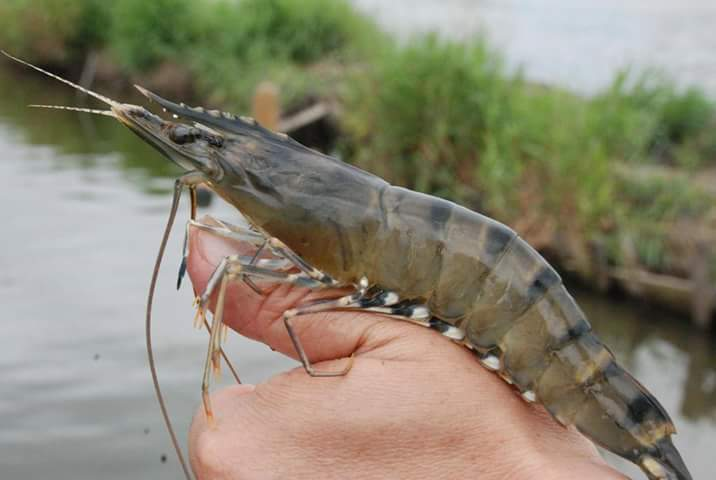
\includegraphics{graphics/Figure-2.jpg}
\caption{Figure 2 : Penaeus monodon}
\end{figure}

\hypertarget{habitat}{%
\subsection{Habitat}\label{habitat}}

Penaeus monodon is found at depths from 0 to 110 m, inhabiting bottom
mud and sand. Giant tiger prawn live in brackish, estuarine (juveniles)
and marine (adults) environments (FAO, 1980). In its natural range, P.
monodon frequents water temperatures of 18--34.5 ºC and salinitiesof
5--45 ppt (Branford, 1981; Chen, 1990). It is even grown commercially at
salinities of 1--5 ppt (Musig and Boonnom, 1998). Penaeus monodon
appears to select muddy mangrove channels and often associates with
marginal or floating vegetation (FAO, 2018).

\hypertarget{reproduction}{%
\subsection{Reproduction}\label{reproduction}}

Wild males produce spermatozoa from around 35 g BW and females becomes
gravid from 70 g. Mating occurs at night, shortly after moulting, while
the cuticle is still soft, and sperm are subsequently kept in a
spermatophore (sac) inserted inside the closed thelycum of the female.
Females of P. monodon are highly fecund, with gravid individuals
producing as many as 500 000 to 750 000 eggs. Spawning occurs at night
and fertilization is external, with females releasing sperm from the
thelycum as eggs are released in offshore waters. Nauplii hatch 12--15 h
after fertilization (FAO, 2018).

\hypertarget{immunity}{%
\subsection{Immunity}\label{immunity}}

The first immune process is the recognition of invading microorganisms,
which is mediated by the haemocytes and by plasmatic proteins. The
recognition molecules may interact with and activate the haemocytes,
which play an important and central role in host defense. The
non-self-recognition factors activate several immediate defense systems
mediated by the haemocytes. The innate immune response of arthropods
also relies upon the production of antimicrobial peptides that are
active against a large range of pathogens. Expression of the immune
effector encoding genes during the response to infections or to immune
stimulations will take place in defense reactions against some specific
harmful pathogens (Bachre, 2000).

\hypertarget{shrimp-cultivation}{%
\subsection{Shrimp cultivation}\label{shrimp-cultivation}}

\hypertarget{traditional-culture-system}{%
\subsubsection{Traditional culture system}\label{traditional-culture-system}}

Shrimp are cultured under this type of management with virtually no cost
or very little cost. Only a few shrimp PL are released in the gher. No
fertilizer or supplementary feed are used in the gher, shrimp fully
depend on natural food present in the gher. Besides, neither any
initiatives are taken nor any technological aspects of farming are
considered in extensive culture method. As a result, only 0.5 kg of
shrimp per decimal are produced annually in the gher. Example can be
given as releasing shrimp PL in the gher without any calculation and not
following gradual steps of shrimp culture and harvesting shrimp
irregularly. Shrimp Pl are stocked at the rate of 10,000-- 15,000 per ha
and fry of other fishes also enter in to the gher with tidal water.
Under this culture system, the survival of shrimp is 30 and per ha
production is 150 kg.

\hypertarget{improved-traditional}{%
\subsubsection{Improved traditional}\label{improved-traditional}}

A little improved culture management, where shrimp PL are stocked at
relatively low density after removing aquatic weed and weed fish /
predatory fish. In addition to irregular fertilizer and feed
application, other activities of planned shrimp culture are also
performed irregularly. Presently, this type of culture management is
most commonly practiced in our country and the shrimp production in this
method is near about 1 kg / dec annually. In the improved traditional ha
stocking density is 15,000 -- 30,000 and per ha shrimp production is 400
-- 500 kg. In the case, the survival of shrimp PL is 50 -- 60 \%.

\hypertarget{semi--intensive}{%
\subsubsection{Semi- intensive}\label{semi--intensive}}

In the semi intensive culture system, the necessary renovation of the
water body, complete control of predatory and weed fish, medium stocking
density, regular fertilizer and handmade feed application, partial
harvesting and restocking after 3-4 months of fry stocking and if
necessary water exchange and supply of oxygen (aeration) are performed.
That is, some modern technologies of shrimp culture are followed under
semi-intensive culture system. Under this type of culture management,
per decimal annual shrimp production may reach 1.5 kg or little more
than that. Under this culture method, per ha stocking density is 9,000
-- 10,000 and per ha production is 450 -- 550 kg. In the case, the
survival of shrimp PL is 70 \%.

\hypertarget{ultra-intensive}{%
\subsubsection{Ultra-intensive}\label{ultra-intensive}}

The culture of shrimp using very advanced technology after costly
infrastructural restoration as necessary is known as intensive culture
system. It requires high investment and rigorous labor. Although
intensive culture system is highly profitable, it has high risk with
potential negative impact on the environment. In this system per ha
stocking density is 50,000 -- 60,000 (if ther is no aerator) and 100,000
(if there is aerator) and the production is 1200 -- 1500 kg. In the
case, the survival of shrimp PL is 80 - 90 \%. (CSISA-BD project, World
Fish, 2011).

\hypertarget{effect-of-salinity-in-shrimp-culture}{%
\subsection{Effect of salinity in shrimp culture}\label{effect-of-salinity-in-shrimp-culture}}

Tiger shrimp Penaeus monodon has a tolerance of a wide range of salinity
from 1 psu to 57 psu and a suitable salinity range of 10 psu to 35 psu
(Liao, 1986). In practice, farmers believe that the growth of shrimp in
lower salinity water is better than in seawater and they are likely to
add freshwater to lower the salinity levels (Wang and Chen, 2006).
However, there is no obvious evidence which showed that growth benefits
could result from such low-salinity-acclimation practices and, in fact,
why and to what degree salinity can affect growth rate and food
conversion efficiency of juvenile P. monodon is still uncertain. (Ye et
al., 2009)

\hypertarget{research-gap}{%
\subsection{Research gap}\label{research-gap}}

The aquaculture research community and the aquafeeds industry have long
recognized and anticipated issues impacting the sustainability of fish
meal in aquafeeds (Barrows and Hardy, 2001). In many countries several
studies have been conducted on researching and developing aquafeeds that
use alternative protein ingredients, particularly plant-derived proteins
(Gatlin et al., 2007). By doing this again we are creating pressure on
human plant food sources, which is a question of global food security
and sustainability. Despite of that we have a huge ocean resources which
have been remained totally untouched. Presently, scientists are thinking
on using huge ocean microbial biomass diversity as the alternative
source of fish meal. However, a little literature has been found on
protein supplementation in shrimp feed with microbial proteins and its
suitability in application at different salinities.

\hypertarget{methodology}{%
\chapter{Methodology}\label{methodology}}

\hypertarget{study-area-and-period}{%
\section{Study area and period}\label{study-area-and-period}}

This study was conducted in Water Chemistry Laboratory of Fisheries and Marine Resource Technology, Khulna University, Bangladesh. The experiment was continued for six weeks from October to November.

\hypertarget{experimental-animal}{%
\section{Experimental Animal}\label{experimental-animal}}

This experiment was a feed trial in tank culture of P. monodon for one and half month. P. monodon juvenile was collected from farmer's nursery pond of Bagerhat District. The animals were transported to Water Chemistry Laboratory and stocked into experimental tanks. After acclimatization at different salinities for 5 days the experiment was subjected to treat with different feeds.

\hypertarget{experimental-tank-set-up-and-salinity-adjustment}{%
\section{Experimental tank set up and salinity adjustment}\label{experimental-tank-set-up-and-salinity-adjustment}}

Newly purchased transparent plastic tanks of 30 L water capacity were used for this experiment. The tanks water volume were maintained up to 25 L throughout the experiment. All the tanks under different treatments were distributed randomly in the laboratory. Different salinity levels were adjusted by calculating using the formula, S1V1 = S2V2. Brine water of 120 ppt was used to adjust the salinity.

\hypertarget{experimental-design}{%
\section{Experimental Design}\label{experimental-design}}

The experimental trial were conducted on 30 L transparent plastic tanks. The animals were cultured in four different salinity levels (5, 10, 15, and 20 ppt) with four different experimental feeds (F1, F2, F3, and F4). We also planned to culture the juvenile at 0 ppt, but after 3 days of stocking all the animals were dead. All the tanks were well set up with continuous aeration and covered with plastic lids to avoid unwanted contamination from outside. Each of the treatment was repeated in three tanks with equal facilities.

Table 3.1 Layout of the Experiment

\begin{longtable}[]{@{}
  >{\raggedright\arraybackslash}p{(\columnwidth - 8\tabcolsep) * \real{0.1127}}
  >{\raggedright\arraybackslash}p{(\columnwidth - 8\tabcolsep) * \real{0.2113}}
  >{\raggedright\arraybackslash}p{(\columnwidth - 8\tabcolsep) * \real{0.2254}}
  >{\raggedright\arraybackslash}p{(\columnwidth - 8\tabcolsep) * \real{0.2254}}
  >{\raggedright\arraybackslash}p{(\columnwidth - 8\tabcolsep) * \real{0.2254}}@{}}
\toprule()
\begin{minipage}[b]{\linewidth}\raggedright
Feed
\end{minipage} & \begin{minipage}[b]{\linewidth}\raggedright
Salinity 5ppt
\end{minipage} & \begin{minipage}[b]{\linewidth}\raggedright
Salinity 10ppt
\end{minipage} & \begin{minipage}[b]{\linewidth}\raggedright
Salinity 15ppt
\end{minipage} & \begin{minipage}[b]{\linewidth}\raggedright
Salinity 20ppt
\end{minipage} \\
\midrule()
\endhead
& S\textsubscript{5} & S\textsubscript{5} & S\textsubscript{5} & S\textsubscript{10} \\
F1 (A) & R\textsubscript{1} & R\textsubscript{2} & R\textsubscript{3} & R\textsubscript{1} \\
F2 (B) & R\textsubscript{1} & R\textsubscript{2} & R\textsubscript{3} & R\textsubscript{1} \\
F3 (C) & R\textsubscript{1} & R\textsubscript{2} & R\textsubscript{3} & R\textsubscript{1} \\
F4 (D) & R\textsubscript{1} & R\textsubscript{2} & R\textsubscript{3} & R\textsubscript{1} \\
\bottomrule()
\end{longtable}

\hypertarget{feeding-management}{%
\section{Feeding management}\label{feeding-management}}

During the experiment the shrimps were fed to satiety twice daily, seven days a week for the six week duration of the experiment. The feed ration allocation was determined by feeding to slight excess (110-120\% of satiation). Initial feed rate was 6\% of tank biomass / daily (initial 1.2g a day).

Table 3.2 List of different feed ingredients of four different diets.

\begin{longtable}[]{@{}
  >{\raggedright\arraybackslash}p{(\columnwidth - 12\tabcolsep) * \real{0.1429}}
  >{\raggedright\arraybackslash}p{(\columnwidth - 12\tabcolsep) * \real{0.1429}}
  >{\raggedright\arraybackslash}p{(\columnwidth - 12\tabcolsep) * \real{0.1429}}
  >{\raggedright\arraybackslash}p{(\columnwidth - 12\tabcolsep) * \real{0.1429}}
  >{\raggedright\arraybackslash}p{(\columnwidth - 12\tabcolsep) * \real{0.1429}}
  >{\raggedright\arraybackslash}p{(\columnwidth - 12\tabcolsep) * \real{0.1429}}
  >{\raggedright\arraybackslash}p{(\columnwidth - 12\tabcolsep) * \real{0.1429}}@{}}
\toprule()
\begin{minipage}[b]{\linewidth}\raggedright
Diet
\end{minipage} & \begin{minipage}[b]{\linewidth}\raggedright
Moisture (\%)
\end{minipage} & \begin{minipage}[b]{\linewidth}\raggedright
Crude Lipid (\%)
\end{minipage} & \begin{minipage}[b]{\linewidth}\raggedright
Crude Protein (\%)
\end{minipage} & \begin{minipage}[b]{\linewidth}\raggedright
Ash (\%)
\end{minipage} & \begin{minipage}[b]{\linewidth}\raggedright
Crude Fibre (\%)
\end{minipage} & \begin{minipage}[b]{\linewidth}\raggedright
Carbohydrate (\%)
\end{minipage} \\
\midrule()
\endhead
F1 & 15.61 & 7.17 & 38.09 & 10.57 & 4.20 & 24.36 \\
F2 & 14.91 & 6.70 & 37.00 & 12.43 & 5.20 & 23.76 \\
F3 & 13.67 & 6.77 & 39.70 & 9.44 & 4.30 & 26.12 \\
F4 & 13.97 & 7.33 & 40.46 & 7.29 & 5.66 & 25.29 \\
\bottomrule()
\end{longtable}

Uneaten feed was scored (counted) in each tank first thing in the morning prior to feeding, with the scoring used to estimate the amount of uneaten feed and used to adjust the afternoon ration (as per table below). A small set rate was fed to each tank in the morning after scoring (feed 0.3g in AM), the remaining individually adjusted ration was offered at 4pm. Bulk feed was kept in the freezer except when weighing feed.

Table 3.3 Feeding adjustment table.

\begin{longtable}[]{@{}ll@{}}
\toprule()
Pellet Count in AM & Adjustment \\
\midrule()
\endhead
30 + Pellets & Decrease PM ration by \textasciitilde0.3g \\
1 to \textasciitilde30 Pellets & No adjustment \\
No pellets & Increase PM ration by \textasciitilde0.3g \\
\bottomrule()
\end{longtable}

\hypertarget{sampling-and-growth-measurement}{%
\section{Sampling and growth measurement}\label{sampling-and-growth-measurement}}

The weight of shrimp was measured every seven days interval by collecting all the individuals from all the tanks by using scoop net. The weight of the shrimp was taken by an electronic weight measuring balance. The growth parameters will be calculated by the following equations:

Weight Gained (WG) = Final weight -- Initial weight. (Biswas et al., 2012)

Daily weight gain (DWG) (g/day) = \(\frac{{(W_t - W_0)}}{t}\), where \(t\) is the duration of the growth interval (Ghosh et al., 2016)

Daily growth rate (DGR) = \(\frac{{\text{{Weight gained}}}}{{\text{{No. of days}}}} \times 100\) (Rebecca \& Bhavan, 2014)

Weight gain (\%) or Relative Growth Rate (RGR) = \(\frac{{(Final weight - Initial weight)}}{{Initial weight}} \times 100\) (Thimmurugan \& Subramanian, 2004)

Specific growth rate (SGR) = \(\frac{{\ln(W_t) - \ln(W_0)}}{t} \times 100\) (Thimmurugan \& Subramanian, 2004)

Survival rate (SR) \% = \(\frac{{\text{{No. of live prawn}}}}{{\text{{No. of prawn introduced}}}} \times 100\) (Thimmurugan \& Subramanian, 2004)

\hypertarget{data-analysis}{%
\section{Data analysis}\label{data-analysis}}

The data obtained during the experiment was statistically analyzed using Microsoft Excel 10.0, SPSS 25.0 version. Multivariate analysis of variance was done to compare the means of growth data under different treatments.

\hypertarget{results}{%
\chapter{Results}\label{results}}

\hypertarget{growth-performance-of-p.-monodon}{%
\section{\texorpdfstring{Growth performance of \emph{P. monodon}}{Growth performance of P. monodon}}\label{growth-performance-of-p.-monodon}}

The result of this study demonstrated that the maximum percent specific
growth rate was found in tank S5F2 (1.144±1.19) and the minimum was
found to be -0.364±0.53 in tank S10F3 (Table 4.1). In this experiment we
found a significant effect of feeds and salinities on the \%SGR in S10F1,
S10F2, S10F3 and S10F4 compared to other treatment groups (P\textless0.05). The
result of this study did not reveal a significant different in the DWG
among the treatments. However, the higher DWG was found in S5F4
(0.750±0.01) and it was lower in S15F3 (0.000±0.10). Similarly, no
significant differences was observed in DGR as well as in \%RGR values.
The maximum DGR and RGR was found in S15F2, 10.760±0.08 and
378.143±26.03 respectively. However, it was minimum in S10F1,
-0.253±0.53 and -4.553±20.68 respectively. In addition, initial and
final body weight of shrimp was found S10F1, 1.829±0.22 and 2.295±0.56
respectively and was minimum in S20F3, 1.023±.08 and in S5F2,
1.211±0.11. There is no significance differences in initial and final
body weight. In case of weight gain, it was higher in S10F3, 4.842±.04
and minimum in S15F3, -0.014±2.72 (Table 3.1).

\hypertarget{effect-of-feeds-and-salinities-on-combined-dependent-variables}{%
\section{Effect of feeds and salinities on combined dependent variables}\label{effect-of-feeds-and-salinities-on-combined-dependent-variables}}

Different multivariate test statistics (e.g.~Pillai's Trace, Wilks'
Lambda, Hotelling's Trace and Roy's Largest Root) showed statistical
significance of different effects of the independent variable salinity
on the combined dependent variable, F(15, 77.697) = 1.808, p = 0.048;
Wilks' Λ = 0.438. The most commonly recommended multivariate statistic
to use is Wilks' Lambda has been used for interpretation of the results.
There was no statistically significant effect was observed in the
interaction effect between treatment and salinity on the combined
dependent variables, F(45, 128.354) = 0.946, p = .573; Wilks' Λ = .278.
Similarly, four feed treatments did not show any significant differences
on the combined dependent variables, F(15, 77.697) = 1.071, p = 0.397 ;
Wilks' Λ =0.595 (Table 3.2).

Table 4.1 Growth parameters (W0, Wt, WG, \%SGR, DWG, DGR, \%RGR) (mean ±
standard error) of P. monodon treated with four different experimental
diets and at different salinities. Different superscript letters (effect
of feed) and estarics (effect of salinities) indicate significant
difference among the treatments (Two-way multivariate analysis of
variance, P\textless0.05).

\begin{longtable}[]{@{}
  >{\raggedright\arraybackslash}p{(\columnwidth - 14\tabcolsep) * \real{0.1250}}
  >{\centering\arraybackslash}p{(\columnwidth - 14\tabcolsep) * \real{0.1250}}
  >{\centering\arraybackslash}p{(\columnwidth - 14\tabcolsep) * \real{0.1250}}
  >{\centering\arraybackslash}p{(\columnwidth - 14\tabcolsep) * \real{0.1250}}
  >{\centering\arraybackslash}p{(\columnwidth - 14\tabcolsep) * \real{0.1250}}
  >{\centering\arraybackslash}p{(\columnwidth - 14\tabcolsep) * \real{0.1250}}
  >{\centering\arraybackslash}p{(\columnwidth - 14\tabcolsep) * \real{0.1250}}
  >{\raggedright\arraybackslash}p{(\columnwidth - 14\tabcolsep) * \real{0.1250}}@{}}
\toprule()
\begin{minipage}[b]{\linewidth}\raggedright
Treatment
\end{minipage} & \begin{minipage}[b]{\linewidth}\centering
W0
\end{minipage} & \begin{minipage}[b]{\linewidth}\centering
Wt
\end{minipage} & \begin{minipage}[b]{\linewidth}\centering
WG
\end{minipage} & \begin{minipage}[b]{\linewidth}\centering
\%SGR
\end{minipage} & \begin{minipage}[b]{\linewidth}\centering
DWG
\end{minipage} & \begin{minipage}[b]{\linewidth}\centering
DGR
\end{minipage} & \begin{minipage}[b]{\linewidth}\raggedright
\%RGR
\end{minipage} \\
\midrule()
\endhead
S5F1 & 1.279±.03 & 1.782±.36 & 1.656±.95a* & .652±.39a* & .037±.02a* & 3.681±2.11a* & 126.941±70.46a* \\
S5F2 & 1.223±.14 & 1.211±.11 & -.114±.82a* & 1.144±1.19a* & 0.075±.08a* & 7.507±8.15a* & 188.389±194.20a* \\
S5F3 & 1.199±.07 & 1.564±.10 & 3.499±.32a* & 0.802±.28a* & 0.079±.03a* & 7.919±3.45a* & 294.576±136.95a* \\
S5F4 & 1.121±.20 & 1.425±.20 & 2.907±.63a* & 0.803±.31a* & 0.750±.01a* & 7.500±3.37a* & 250.706±87.19a* \\
S10F1 & 1.829±.22 & 2.295±.56 & 3.378±3.67a* & -.011±.05a** & 0.003±.03a* & -0.253±.53a* & -4.553±20.68a* \\
S10F2 & 1.402±.05 & 1.496±.21 & 0.544±1.22a* & 0.104±.23a** & 0.012±.02a* & 1.208±2.70a* & 32.111±85.83a* \\
S10F3 & 1.293±.09 & 1.813±.09 & 4.842±.04a* & -.364±.53a** & .004±.06a* & .437±2.17a* & 11.668±72.83a* \\
S10F4 & 1.566±.22 & 1.940±.20 & 3.254±.93a* & .839±.49a** & 0.098±.01a* & 9.810±6.30a* & 306.101±169.03a* \\
S15F1 & 1.242±.04 & 1.798±.18 & 3.563±1.56a* & 0.588±.05a* & 0.078±0.0a* & 7.775±.71a* & 291.503±20.03a* \\
S15F2 & 1.341±.41 & 1.215±.28 & 0.197±0.98a* & 0.757±.06a* & 0.108±0.0a* & 10.760±.08a* & 378.143±26.03a* \\
S15F3 & 1.493±.17 & 1.574±.16 & -.014±2.72a* & 0.062±.51a* & 0.000±0.10a* & -.031±6.04a* & 36.287±167.92a* \\
S15F4 & 1.411±.11 & 1.828±.43 & 3.81±3.19a* & 0.574±.32a* & 0.067±.00a* & 6.673±4.02a* & 294.078±180.06a* \\
S20F1 & 1.233±.19 & 1.826±.52 & 3.375±1.52a* & 0.574±0.18a* & 0.065±.04a* & 6.459±1.39a* & 293.159±104.77a* \\
S20F2 & 1.371±.17 & 2.170±72 & 4.415±2.84a* & 0.502±0.18a* & 0.072±.02a* & 7.230±2.06a* & 223.903±75.89a* \\
S20F3 & 1.023±.08 & 1.353±.22 & 3.003±1.81a* & 0.480±0.39a* & 0.085±.07a* & 8.474±7.08a* & 256.075±199.77a* \\
S20F4 & 1.204±10 & 1.306±.07 & 1.417±1.33a* & 0.189±.31a* & 0.032±.03a* & 3.171±2.96a* & 137.960±113.45a* \\
\bottomrule()
\end{longtable}

\emph{Note that, W0= Initial weight, Wt= Final weight ,WG= Weight gain, \%SGR=
Percentage specific growth rate, DWG= Daily weight gain, DGR= Daily
growth rate, \%RGR= Percentage relative growth rate.} S5= Salinity 5 ppt,
S10= Salinity 10 ppt, S15= Salinity 15 ppt, S20=Salinity 20ppt. *F1=
Feed 1, F2= Feed 2, F3= Feed 3, F4= Feed 4.

\begin{longtable}[]{@{}
  >{\raggedright\arraybackslash}p{(\columnwidth - 12\tabcolsep) * \real{0.1429}}
  >{\raggedright\arraybackslash}p{(\columnwidth - 12\tabcolsep) * \real{0.1429}}
  >{\raggedright\arraybackslash}p{(\columnwidth - 12\tabcolsep) * \real{0.1429}}
  >{\raggedright\arraybackslash}p{(\columnwidth - 12\tabcolsep) * \real{0.1429}}
  >{\raggedright\arraybackslash}p{(\columnwidth - 12\tabcolsep) * \real{0.1429}}
  >{\raggedright\arraybackslash}p{(\columnwidth - 12\tabcolsep) * \real{0.1429}}
  >{\raggedright\arraybackslash}p{(\columnwidth - 12\tabcolsep) * \real{0.1429}}@{}}
\toprule()
\begin{minipage}[b]{\linewidth}\raggedright
Effect
\end{minipage} & \begin{minipage}[b]{\linewidth}\raggedright
\end{minipage} & \begin{minipage}[b]{\linewidth}\raggedright
Value
\end{minipage} & \begin{minipage}[b]{\linewidth}\raggedright
F
\end{minipage} & \begin{minipage}[b]{\linewidth}\raggedright
Hypothesis df
\end{minipage} & \begin{minipage}[b]{\linewidth}\raggedright
Error df
\end{minipage} & \begin{minipage}[b]{\linewidth}\raggedright
Sig.
\end{minipage} \\
\midrule()
\endhead
Intercept & Pillai's Trace & .594 & 14.653b & 3.000 & 30.000 & .000 \\
& Wilks' Lambda & .406 & 14.653b & 3.000 & 30.000 & .000 \\
& Hotelling's Trace & 1.465 & 14.653b & 3.000 & 30.000 & .000 \\
& Roy's Largest Root & 1.465 & 14.653b & 3.000 & 30.000 & .000 \\
Treatment & Pillai's Trace & .200 & .763 & 9.000 & 96.000 & .651 \\
& Wilks' Lambda & .812 & .727 & 9.000 & 73.163 & .683 \\
& Hotelling's Trace & .217 & .692 & 9.000 & 86.000 & .715 \\
& Roy's Largest Root & .107 & 1.144c & 3.000 & 32.000 & .346 \\
Salinity & Pillai's Trace & .499 & 2.126 & 9.000 & 96.000 & .034 \\
& Wilks' Lambda & .563 & 2.165 & 9.000 & 73.163 & .034 \\
& Hotelling's Trace & .668 & 2.129 & 9.000 & 86.000 & .035 \\
& Roy's Largest Root & .419 & 4.465c & 3.000 & 32.000 & .010 \\
Treatment * Salinity & Pillai's Trace & .553 & .804 & 27.000 & 96.000 & .737 \\
& Wilks' Lambda & .533 & .786 & 27.000 & 88.258 & .757 \\
& Hotelling's Trace & .724 & .769 & 27.000 & 86.000 & .778 \\
& Roy's Largest Root & .440 & 1.566c & 9.000 & 32.000 & .168 \\
\bottomrule()
\end{longtable}

\hypertarget{effect-of-feeds-and-salinities-on-individual-dependent-variables}{%
\section{Effect of feeds and salinities on individual dependent variables}\label{effect-of-feeds-and-salinities-on-individual-dependent-variables}}

Tests of between-subjects effects of multivariate analysis of variance
showed that there was no significant difference in the interaction
effect between treatment and salinity on Wt, F(9,.286) =.871, p = .560;
Type III Sum of Squares = 2.575; WG, F(9, 8.945) = 0.888, p = 0.546;
Type III Sum of Squares = 80.504; SGR, F(9, 0.295) = 0.523, p = 0.847;
Type III Sum of Squares = 2.654; on DWG, F(9, 0.04) = 0.888, p = 0.546;
Type III Sum of Squares = 0.040; on DGR, F(9, 44.172) = 0.888, p =
0.546; Type III Sum of Squares = 397.549 and for RGR, F(9, 46382.390) =
1.019, p = .446; Type III Sum of Squares = 417441.510 (Table 4.3).

Different feeds had no significant effect on the growth Penaeus monodon
(e.g.Wt, DW, SGR, DWG, DGR, RGR) with the F and P values; for Wt,
F(3,.390) =1.186, p = .330; Type III Sum of Squares = 1.169; WG, F(3,
8.049) = 0.799, p = 0.503; Type III Sum of Squares = 24.147; SGR, F(3,
.369) = .655, p = .586; Type III Sum of Squares = 1.108; for DWG, F(3,
0.002) = .475, p = .702; Type III Sum of Squares = 0.007; for DGR, F(3,
23.639) = .475, p = .702; Type III Sum of Squares = 70.916 and for RGR,
F(3, 20912.412) = .459, p = .713; Type III Sum of Squares = 62737 (Table
4.3).

Similarly, salinities also did not have significant effect on the growth
of Penaeus monodon (e.g.~Wt, DW, SGR, DWG, DGR, RGR) with the F and P
values; for Wt, F(3,.326) =.992, p = .409; Type III Sum of Squares =
.977; WG, F(3, 4.787) = 0.475, p = 0.702; Type III Sum of Squares =
14.361 for SGR, F(3, 1.014) = 1.799, p = .167; Type III Sum of Squares =
3.043; for DWG, F(3, 0.004) = .799, p = .503; Type III Sum of Squares =
0.012 ; for DGR, F(3, 39.748) = .799, p = .503Type III Sum of Squares =
119.243 and for RGR, F(3, 65256.710) = 1.434 p = .251; Type III Sum of
Squares = 195770.129 (Table 4.3).

Table 4.3 Effect of independent variables and its interactions on the individual dependent variables
(Two-way multivariate analysis of variance, P\textless0.05).

\begin{longtable}[]{@{}
  >{\raggedright\arraybackslash}p{(\columnwidth - 12\tabcolsep) * \real{0.2188}}
  >{\raggedright\arraybackslash}p{(\columnwidth - 12\tabcolsep) * \real{0.2083}}
  >{\raggedright\arraybackslash}p{(\columnwidth - 12\tabcolsep) * \real{0.2500}}
  >{\raggedright\arraybackslash}p{(\columnwidth - 12\tabcolsep) * \real{0.0521}}
  >{\raggedright\arraybackslash}p{(\columnwidth - 12\tabcolsep) * \real{0.1354}}
  >{\raggedright\arraybackslash}p{(\columnwidth - 12\tabcolsep) * \real{0.0729}}
  >{\raggedright\arraybackslash}p{(\columnwidth - 12\tabcolsep) * \real{0.0625}}@{}}
\toprule()
\begin{minipage}[b]{\linewidth}\raggedright
Source
\end{minipage} & \begin{minipage}[b]{\linewidth}\raggedright
Dependent Variable
\end{minipage} & \begin{minipage}[b]{\linewidth}\raggedright
Type III Sum of Squares
\end{minipage} & \begin{minipage}[b]{\linewidth}\raggedright
df
\end{minipage} & \begin{minipage}[b]{\linewidth}\raggedright
Mean Square
\end{minipage} & \begin{minipage}[b]{\linewidth}\raggedright
F
\end{minipage} & \begin{minipage}[b]{\linewidth}\raggedright
Sig.
\end{minipage} \\
\midrule()
\endhead
Corrected Model & SGR & 6.804a & 15 & .454 & .805 & .665 \\
& DWG & .059b & 15 & .004 & .788 & .681 \\
& DGR & 587.709c & 15 & 39.181 & .788 & .681 \\
& RGR & 675948.875d & 15 & 45063.258 & .990 & .488 \\
Intercept & SGR & 11.104 & 1 & 11.104 & 19.699 & .000 \\
& DWG & .146 & 1 & .146 & 29.415 & .000 \\
& DGR & 1462.601 & 1 & 1462.601 & 29.415 & .000 \\
& RGR & 1821744.322 & 1 & 1821744.322 & 40.022 & .000 \\
Treatment & SGR & 1.108 & 3 & .369 & .655 & .586 \\
& DWG & .007 & 3 & .002 & .475 & .702 \\
& DGR & 70.916 & 3 & 23.639 & .475 & .702 \\
& RGR & 62737.235 & 3 & 20912.412 & .459 & .713 \\
Salinity & SGR & 3.043 & 3 & 1.014 & 1.799 & .167 \\
& DWG & .012 & 3 & .004 & .799 & .503 \\
& DGR & 119.243 & 3 & 39.748 & .799 & .503 \\
& RGR & 195770.129 & 3 & 65256.710 & 1.434 & .251 \\
Treatment * Salinity & SGR & 2.654 & 9 & .295 & .523 & .847 \\
& DWG & .040 & 9 & .004 & .888 & .546 \\
& DGR & 397.549 & 9 & 44.172 & .888 & .546 \\
& RGR & 417441.510 & 9 & 46382.390 & 1.019 & .446 \\
Error & SGR & 18.038 & 32 & .564 & & \\
& DWG & .159 & 32 & .005 & & \\
& DGR & 1591.150 & 32 & 49.723 & & \\
& RGR & 1456597.274 & 32 & 45518.665 & & \\
Total & SGR & 35.946 & 48 & & & \\
& DWG & .364 & 48 & & & \\
& DGR & 3641.459 & 48 & & & \\
& RGR & 3954290.471 & 48 & & & \\
Corrected Total & SGR & 24.842 & 47 & & & \\
& DWG & .218 & 47 & & & \\
& DGR & 2178.859 & 47 & & & \\
& RGR & 2132546.149 & 47 & & & \\
\bottomrule()
\end{longtable}

\hypertarget{discussion}{%
\chapter{Discussion}\label{discussion}}

Most penaeid shrimps are known to be euryhaline species growing in a wide range of salinities. P.
monodon exhibits hyper-osmotic regulation at low salinity levels, and exhibits hypo-osmotic
regulation at high salinity levels (Cheng and Liao, 1986). However, the low survival rate at 5 ppt
found in this study, which was similar to the result obtained with postlarvae by Cawthorne et al.
(1983). The authors argued that the adaptation ability of P. monodon to low salinity is relatively
weak.

Abnormal molting may also increase the opportunities of cannibalism due to weakness during
molting, and anyway would usually be lethal for shrimps. On the other hand, as shown in our
results, although low salinity enhanced molting, it did not accelerate growth rate but had adverse
effects on the growth of P. monodon. In fact, similar observations have been verified in other
crustaceans (Allan and Maguire, 1992; Vuayan and Diwan, 1995; Romano and Zeng, 2006).
Considering the fact, the mortality was found in a few tank. In this experiment, the salinity have a
significant difference on the variation of combined dependent variable. (P\textless{} 0.05) (Table. 4.2).
Although, all the experimental tanks were placed in the same laboratory, but this effect might be
due to different salinities that might have effect on the psychological responses such as increasing
or decreasing the dissolve oxygen consumption. However, different feeds, and feed-salinity
interaction were found to have no significant effect on the variation of combined dependent
variables (P\textgreater0.05) (Table 3). On the other hand, test of between subject effects demonstrated that
different feeds, salinities, and interaction of feeds and salinities had no significant effect on the
individual dependent variable in different tanks. (P\textgreater0.05) (Table 4.3). This phenomenon was
observed might be due to lower adaptability of shrimp with newly formulated feed, different level
of salinities, and off course due to environmental fluctuations as well as seasonal dynamics during
the experimental period.

The costs of formulated feed and labor associated with feeding are a major component of the cost
of cultured shrimp production (Lawrence and Lee, 1997). It is well established that the nutrient
content of the feed will influence growth, survival and the amount of metabolic and excreted waste
products entering the system. (Smith, Burford, \& Tabrett, 2002)

In the present study, the specific growth rate was ranged from 1.144±1.19 to -0.364±0.53. In this
experiment we found a significant effect of feeds and salinities on the \%SGR in S10F1, S10F2,
S10F3 and S10F4 compared to other treatment groups (P\textless0.05). In addition, according to test of
between subjects effects, different feeds and salinities had significant effect on the \% SGR in
different tanks (Table 4.3). However, interaction of this two factors did not have any influence on
the individual dependent variable, \%SGR (P\textless0.05) (Table 4.3). Variation of \%SGR in different
tanks might be due to variations in salinities which might influenced the respiratory metabolism
of Penaeus monodon.(Ye et al., 2009).

No significant differences was observed in DGR as well as in \%RGR values. DGR was raged from
10.760±0.08 to -0.253±0.53 and RGR was raged 378.143±26.03 to -4.553±20.68. The results of
the current experiments indicated that salinity can have an immediate and significant effect on
survival, and growth. A salinity range outside 20--30 ppt will increase energy channeled to
respiration, excretion and exuviae. Thus, a salinity range between 20 and 30 ppt is recommended
for the culture of juvenile P. monodon. This conclusion has significant implications for P.
monodon aquaculture, as it can be utilized in farm site selection and salinity maintenance to
maximize commercial productivity.(Ye et al., 2009).

\hypertarget{conclusion-and-recommendation}{%
\chapter{Conclusion and Recommendation}\label{conclusion-and-recommendation}}

\hypertarget{conclusion}{%
\section{Conclusion}\label{conclusion}}

From the present study the following conclusions can be drawn-

\begin{itemize}
\item
  Salinity can have an immediate and significant effect on the growth
  performance of \emph{P. monodon}.
\item
  Different feeds and salinity-feed interaction have no significant
  effect on the growth performance of the cultured species.
\item
  Both feed and salinity have significant effect on the percentage
  specific growth rate (\%SGR) of the cultured species.
\end{itemize}

\hypertarget{recommendation}{%
\section{Recommendation}\label{recommendation}}

\begin{enumerate}
\def\labelenumi{\arabic{enumi}.}
\item
  Environmental uncertainties should be minimized during this type of
  experiment in laboratories.
\item
  Further evaluation on effectiveness of microbial protein in animal
  health should be checked through unraveling their nutritional
  requirements and physiological mechanisms.
\end{enumerate}

\end{document}
